\section{The \resource{} Resource}
\label{sec:rel-graph}


To test the consistency of PLMs, we opt to test their predictions sensitivity to variations patterns for which the same answer is expected. This requires a large set of paraphrased queries. To this end, we create a paraphrase resource that enables us to study this property, which we name \resource{}. \resource{} is a high-quality resource, built by experts. %, and results in a high-quality resource which we hope can contribute to others' work as well.
It contains patterns for 40 relations from the TREx dataset \cite{trex}, with an average of @@ patterns per relation.
Each pattern is represented as a node in an undirected graph, and each edge signifies the type of modification from one pattern to another (e.g. lexical change).
A schematic view of the ``aired on'' relation can be seen in Figure \ref{fig:graph}. 

% All patterns from a specific relation are paraphrases.
% Each pattern entails the main expression for each pattern, but not necessarily the other way around. 
% For example, for the relation of ``aired on'', which describes a TV-series that was aired on some network, the original pattern is: ``\subj{} was aired on \obj{}'' and one of the patterns we create is ``\subj{} was premiered on \obj{}'', which entails the main expression, but not vice versa.


% For instance, the phrase "\subj{} was aired on \obj{}" entails "\obj{} released \subj{}", but not "\subj{} was premiered on \obj{}", although the other direction is entailed.
% \ar{The entailment 'Y released X' doesn't seem correct. Suggestion For instance, the phrase "\subj{} was premiered on \obj{}" entails "\subj{} was aired on \obj{}", but not the other way around.}

\begin{figure}[t!]
\centering

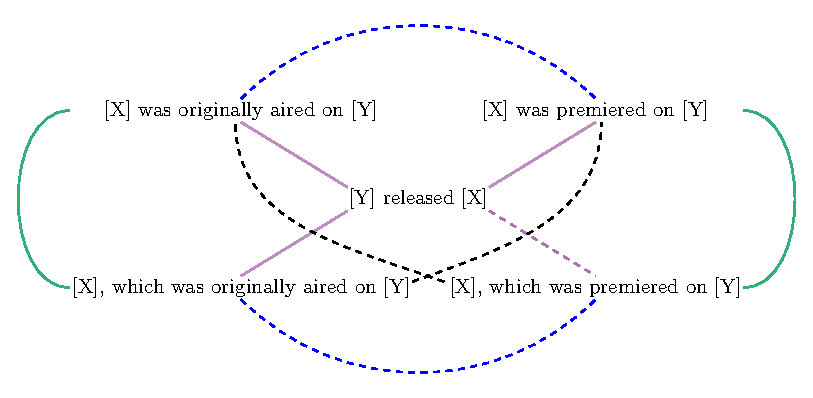
\includegraphics[width=1.\columnwidth]{figures/ent_graph}

\caption{Overview of \resource{}.}
\label{fig:graph}
% \vspace{-6mm}
\end{figure}

% Overall, \resource{} contains @@ different patterns in total for @@ different relations (@@\% paraphrases per relation in average). 
% All of the paraphrases for a particular relation are organized as a directed graph to indicate the entailment relation between two patterns. 
% Each edge also contains information about the transformation type, e.g. a lexical or syntactic transformation (Examples for each can be seen in Figure \ref{fig:graph}).
%A detailed definition is provided shortly.
% \ye{need to define this.} 
% This information allows us to study the different generalization capabilities of models.
% The nodes of the graph (which account for the phrases), also contain additional information about the number of times that the pattern appeared in Wikipedia, @@ more?. %\ar{will we still have the wikipedia info in the paper?}

\resource{}, was constructed in four steps:
(1) We begin with the patterns provided by LAMA \cite{lama} (one pattern per relation, referred to as base pattern). (2) Then, we augmented that relation with other patterns that are paraphrases of the base pattern. Some of these relations are taken from LPAQA \cite{alpaqa}. However, since its relations were extracted automatically, many do not accurately depict the relation, therefore only a subset of these patterns were used in practice. 
% \nk{should we give a number?}.\ye{I don't think it's necessary}
(3) Then, by using spike \cite{spike}, we searched for additional patterns that appeared in Wikipedia and added them to our resource. This was done by searching for subject and object tuples from the TREx resource and looking at the sentences that contain both. (4) Lastly, we augment additional patterns using the annotators' linguistic expertise, such that they are either paraphrase of the base pattern or entail the base pattern. 
Then, two additional authors went over all the patterns and corrected them, while engaging in a discussion until reaching an agreement, discarding patterns with disagreements.
% \nk{Not sure if the details of this need to be in the main paper or can be moved to the appendix?} \sr{I support moving the technicalities to an appendix and focus here on the properties of the resources and how it is being used.}
% \ye{can decide when we have the full story}
%The entailment edges were also annotated by the same two authors that created the patterns.

\begin{table}[t]
% \small
    \centering
\begin{tabular}{lr}
\toprule
           stat &   values \\
\midrule
      n. graphs &    15 \\
   avg patterns &    19.73 \\
   min patterns &     9 \\
   max patterns &    37 \\
       n. edges &  4821 \\
 edge syntactic &     0.03 \\
   edge lexical &     0.87 \\
      edge both &     0.09 \\
\bottomrule
\end{tabular}
    \caption{Statistics for \resource{}. \ye{numbers are not updates with all the graphs}}
    \label{tab:rel-graph-stats}
\end{table}


\paragraph{Consistency Types}
% \nk{we should change inference types to consistency types} \ye{but the graph is in entailment graph}
To study the consistency against syntactic and lexical variations of models, each edge is augmented with the type of changes performed to reach from one pattern to another. We account for three types of changes: 1) \textit{syntactic}, 2) \textit{lexical} and 3) \textit{determiner}, all binary variables that account for a change of the specific type between two patterns.
\textit{Syntactic} structure is defined as the dependency path between the subject and the object in a given pattern, where the path includes the edge types. Two patterns are considered equal syntactically if the labeled paths are identical.
\textit{Lexical} difference is defined by words difference between two patterns, excluding determiners, punctuation, and symbols. The addition or removal of a preposition does not count as a lexical change.
\textit{Determiner} difference is considered when the patterns' determiners do not fully overlap.


Some statistics of the graphs are presented in Table \ref{tab:rel-graph-stats}, and full statistics per relation are presented in Table \ref{tab:rel-graph-stats-elaborate} in the Appendix.



% \begin{table*}[t]
% \small
    \centering
\resizebox{1\textwidth}{!}{%
\begin{tabular}{llll}
\toprule
           Pattern & Base &  Entailed & Type \\
\midrule
% hi & byw & chao \\
      \textsc{Died-in} & \textsc{Subj} passed away in \textsc{Obj}. & $\Leftrightarrow$ \textsc{Subj} died in OBJ. & lexical \\
       & \textsc{Subj} was murdered at \textsc{Obj}. & $\Rightarrow$ \textsc{Subj} died in \textsc{Obj}. & lexical \& syntactic \\
       & \textsc{Subj} died at \textsc{Obj}. & $\Leftrightarrow$ \textsc{Subj} died in \textsc{Obj}. & lexical \\
       
       \midrule
       
       \textsc{Official-language} & \textsc{Obj} is the official language of \textsc{Subj}. & $\Leftrightarrow$ The official language of \textsc{Subj} is \textsc{Obj}. & syntactic \\
       & In \textsc{Subj} \textsc{Obj} is an official language. & $\Leftrightarrow$ The official language of \textsc{Subj} is \textsc{Obj}.	& \\
       
       \midrule
       
       \textsc{Located-in} & \textsc{Subj} is a county in \textsc{Obj}. & $\Rightarrow$ \textsc{Subj} is located in \textsc{Obj} . & lexical \& syntactic \\
       & \textsc{Subj} district, \textsc{Obj}.	& $\Rightarrow$ \textsc{Subj} is located in \textsc{Obj} . & lexical \& syntactic \\
       
       \midrule
       
       \textsc{Instrument} & \textsc{Subj} was a \textsc{Obj} player. & $\Rightarrow$ \textsc{Subj} plays \textsc{Obj}. & lexical \& syntactic \\
       & \textsc{Subj} played \textsc{Obj} . & $\Leftarrow$ \textsc{Subj} plays \textsc{Obj}. & tense \\
       & \textsc{Obj} sonatas of \textsc{Subj}. & $\Rightarrow$ \textsc{Subj} plays \textsc{Obj}. & lexical \& syntactic \\
       
\bottomrule
\end{tabular}
}
    \caption{Examples of patterns in the \resource{}.}
    \label{tab:rel-graph-examples}
\end{table*}

